\documentclass[11pt,a4paper]{article}
\usepackage[T1]{fontenc}
\usepackage[utf8]{inputenc}
\usepackage[french]{babel}
\usepackage{lmodern}
\usepackage{geometry}
\geometry{margin=2.3cm}
\usepackage{amsmath,amssymb,booktabs,array,multirow}
\usepackage{graphicx}
\usepackage{float}
\usepackage{caption}
\captionsetup{font=small,labelfont=bf}
\usepackage{hyperref}
\usepackage{xcolor}
\usepackage{fancyhdr}
\usepackage{enumitem}
\usepackage{tocloft}
\setlength{\cftbeforesecskip}{2pt}
\setlength{\cftbeforesubsecskip}{0pt}
\renewcommand{\cftsecafterpnum}{\hfill}
\hypersetup{colorlinks=true,linkcolor=blue!45!black,urlcolor=blue!45!black,citecolor=blue!45!black}
\pagestyle{fancy}
\fancyhf{}
\fancyhead[L]{\small Projet 12 --- Exportations agroalimentaires marocaines}
\fancyhead[R]{\small Data Science et commerce international}
\fancyfoot[C]{\thepage}
\setlength{\parskip}{0.35em}
\setlength{\parindent}{0pt}
\newcommand{\todo}[1]{\textcolor{blue!60!black}{\textbf{[À compléter : #1]}}}
\newcommand{\MUSD}{\,\text{M USD}}

\title{\textbf{Prévoir les exportations agroalimentaires marocaines par marché\\[0.3em]
\large Une comparaison de modèles temporels sur le chapitre 08 du Système harmonisé, 2010--2024}}
\author{\todo{Binôme : Nom 1 et Nom 2}}
\date{Année universitaire 2026--2027}

\begin{document}

\begin{titlepage}
\centering
{\Large \todo{Établissement} \par}
\vspace{0.6cm}
{\large Filière : \todo{filière} \quad Module : Data Science appliquée au commerce international\par}
\vspace{1.6cm}
{\Huge\bfseries Exportations agroalimentaires marocaines\par}
\vspace{0.4cm}
{\LARGE Prévoir les ventes de fruits par marché\par}
\vspace{0.8cm}
{\large Projet n° 12 --- rapport scientifique\par}
\vspace{1.4cm}
\begin{tabular}{rl}
Étudiant(e) 1 : & \todo{Nom 1} \\
Étudiant(e) 2 : & \todo{Nom 2} \\
Responsable : & A. Larhlimi \\
Année universitaire : & 2026--2027 \\
Date de remise : & \todo{JJ/MM/AAAA} \\
\end{tabular}
\vfill
{\small Données : UN Comtrade, API publique \emph{preview}, extraction du 31 octobre 2026.\\
Code, données et figures : dépôt du projet (voir annexe~\ref{ann:repro}).}
\end{titlepage}

\section*{Résumé}
\addcontentsline{toc}{section}{Résumé}

Ce rapport étudie la prévision des exportations marocaines de fruits (chapitre 08
du Système harmonisé) vers six marchés européens entre 2010 et 2024. À partir de
l'API publique UN Comtrade, nous construisons un panel de 1\,260 cellules
(marché $\times$ produit HS4 $\times$ année), dont 66,2\,\% sont réellement
observées, et 648 observations exploitables pour la prévision à un an. Trois
familles de modèles --- régression Ridge, forêt aléatoire et gradient boosting ---
sont comparées à une référence naïve de persistance sous validation temporelle
glissante, puis sur un test final 2023--2024 jamais utilisé lors du réglage.
La persistance obtient le meilleur WAPE moyen en validation (0,297) ; la forêt
aléatoire la devance de peu sur le test (0,255 contre 0,262, soit un MASE de
0,971) mais reste derrière en validation (0,314). Le résultat principal est donc
négatif et robuste : à fréquence annuelle, la valeur exportée d'un couple
marché--produit se comporte presque comme une marche aléatoire. Les modèles
apportent en revanche un gain sur les marchés les plus grands et les plus volatils
(Espagne, Pays-Bas, Royaume-Uni). La projection 2025 s'établit à
1\,771\MUSD{} [1\,608 ; 1\,977] pour les six marchés, soit +10,2\,\% par rapport
à 2024.

\vspace{0.6em}
\noindent\textbf{Mots-clés :} exportations agroalimentaires, Maroc, UN Comtrade,
prévision temporelle, validation glissante, WAPE, persistance.

\begin{table}[H]
\centering
\caption{Chiffres clés du projet}\label{tab:chiffres}
\begin{tabular}{lr}
\toprule
Indicateur & Valeur \\
\midrule
Requêtes API / lignes brutes téléchargées & 45 / 1\,058 \\
Panel analytique (marchés $\times$ produits $\times$ années) & 1\,260 cellules \\
Cellules réellement observées & 834 (66,2\,\%) \\
Observations utilisables pour la prévision & 648 \\
Valeur exportée vers les six marchés en 2024 & 1\,607,6\MUSD \\
Croissance 2010--2024 & $\times 4,9$ (TCAM 12,1\,\%) \\
Meilleur WAPE en validation glissante & 0,297 (persistance) \\
WAPE sur le test 2023--2024 & 0,255 (forêt) / 0,262 (persistance) \\
Projection 2025 (intervalle à 80\,\%) & 1\,771\MUSD{} [1\,608 ; 1\,977] \\
\bottomrule
\end{tabular}
\end{table}

\newpage
\tableofcontents
\newpage

\section{Introduction}\label{sec:intro}

\subsection{Contexte économique}

L'agroalimentaire est devenu un pilier des exportations marocaines. Le chapitre 08
du Système harmonisé --- fruits comestibles, agrumes, fruits à coque --- constitue
l'un des premiers postes vendus à l'Union européenne, porté par trois facteurs :
la proximité géographique et logistique, l'accord d'association UE--Maroc qui
ouvre le marché en franchise de droits pour de nombreux produits, et le
décalage saisonnier qui place les récoltes marocaines sur le marché européen en
contre-saison.

La filière reste néanmoins exposée. D'abord à la \emph{concentration} : quelques
marchés et quelques produits pèsent l'essentiel de la valeur. Ensuite à la
\emph{volatilité des prix} : la valeur exportée mélange un effet volume et un
effet prix, et une hausse de valeur n'est pas nécessairement une hausse
d'activité. Enfin à la \emph{concurrence} : l'Espagne, la Turquie et l'Égypte
ciblent les mêmes fenêtres de marché sur les agrumes et les fruits rouges.

Pour un exportateur ou un responsable de filière, la question opérationnelle est
simple : \emph{combien vais-je vendre l'an prochain sur chacun de mes marchés, et
avec quelle incertitude ?} C'est cette question que le projet traite, en la
réduisant à un problème de prévision supervisée.

\subsection{Problématique et hypothèses}

\textbf{Question de recherche.} Peut-on prévoir, à un horizon d'un an, la valeur
exportée d'un couple (marché, produit HS4) et battre une prévision naïve de
persistance ?

Trois hypothèses structurent l'analyse.

\begin{description}[leftmargin=1.2cm,style=nextline]
\item[H1 --- Persistance.] Les valeurs exportées se comportent comme une marche
aléatoire : la meilleure prévision de l'année $t+1$ est la valeur de l'année $t$.
Les modèles d'apprentissage ne doivent pas la battre systématiquement.
\item[H2 --- Déplacement structurel.] La valeur totale progresse, mais la
composition par produit et par marché se déplace : montée des fruits hors
agrumes, recul relatif de la France.
\item[H3 --- Effet prix.] Une partie de la croissance est une croissance en
valeur (prix unitaires) et non en volume.
\end{description}

\subsection{Objectifs mesurables}

\begin{enumerate}[leftmargin=1.2cm]
\item Constituer un panel reproductible de 6 marchés $\times$ 14 produits HS4
$\times$ 15 années, avec journal d'extraction et contrôle de couverture.
\item Comparer trois familles de modèles à une référence naïve sous validation
temporelle stricte, avec les métriques MAE, RMSE et WAPE.
\item Produire une projection 2025 par marché, assortie d'un intervalle
empirique et de réserves explicites sur son usage.
\end{enumerate}

\section{Présentation du jeu de données}\label{sec:data}

\subsection{Source, période et unité d'analyse}

Les données proviennent de la base \textbf{UN Comtrade} (Division statistique des
Nations unies), via l'API publique d'aperçu
\url{https://comtradeapi.un.org/public/v1/preview/C/A/HS}, documentée à l'adresse
\url{https://uncomtrade.org/docs/un-comtrade-api/}. L'extraction a été réalisée
le 31 octobre 2026 par le script \texttt{src/download\_comtrade.py}.

\begin{table}[H]
\centering
\caption{Paramètres de l'extraction UN Comtrade}\label{tab:extraction}
\begin{tabular}{ll}
\toprule
Paramètre & Valeur \\
\midrule
Déclarant (\texttt{reporterCode}) & Maroc, code 504 \\
Flux (\texttt{flowCode}) & Exportations (\texttt{X}) \\
Produits (\texttt{cmdCode}) & HS 08 et positions HS4 0801 à 0814 \\
Partenaires & France 251, Espagne 724, Allemagne 276, Pays-Bas 528, \\
             & Royaume-Uni 826, Italie 380 ; Monde 0 (totaux) \\
Période & 2010--2024, fréquence annuelle \\
Classification & H6 (\emph{Harmonized System} 2017) \\
Valeur & \texttt{primaryValue}, dollars américains courants \\
Contraintes de l'API & 1 période par requête, 500 lignes maximum, sans clé \\
\bottomrule
\end{tabular}
\end{table}

L'unité d'analyse est le triplet (marché de destination, produit HS4, année).
Le choix du HS4 plutôt que du HS2 est délibéré : il isole les agrumes (0805) et
les autres fruits frais (0810), dont les dynamiques sont très différentes.
Le choix de six marchés plutôt que des deux marchés cités dans la fiche
(France et Espagne) est justifié par la taille de l'échantillon : avec deux
marchés et quinze années, un modèle supervisé n'aurait que trente observations
par produit. Les six marchés retenus représentent 75,6\,\% de la valeur exportée
vers le monde en 2024.

\paragraph{Traçabilité.} Chaque requête est journalisée (URL, statut, nombre de
lignes, horodatage UTC) dans \texttt{data/processed/journal\_extractions.csv} et
chaque réponse JSON brute est conservée. Au total : 45 requêtes, 1\,058 lignes
brutes téléchargées, aucune requête en échec.

\subsection{Dictionnaire des variables}

\begin{table}[H]
\centering
\caption{Dictionnaire des variables du panel analytique}\label{tab:variables}
\small
\small
\begin{tabular}{>{\raggedright\arraybackslash}p{3.7cm}>{\raggedright\arraybackslash}p{1.4cm}>{\raggedright\arraybackslash}p{2.3cm}>{\raggedright\arraybackslash}p{5.5cm}}
\toprule
Variable & Type & Unité & Rôle \\
\midrule
\texttt{annee} & entier & année & index temporel \\
\texttt{partnerCode} & entier & code ONU & identifiant du marché \\
\texttt{cmdCode} & texte & code HS4 & identifiant du produit \\
\texttt{valeur\_usd} & réel & USD courants & valeur exportée (variable expliquée) \\
\texttt{poids\_net\_kg} & réel & kilogrammes & volume déclaré \\
\texttt{prix\_unitaire\_usd\_kg} & réel & USD/kg & prix implicite \\
\texttt{monde\_usd} & réel & USD courants & exportations du produit vers le monde \\
\texttt{part\_marche} & réel & 0--1 & poids du marché dans le produit \\
\texttt{declare} & 0/1 & indicatrice & 1 = observé, 0 = imputé \\
\texttt{retenu\_pour\_modele} & 0/1 & indicatrice & couverture $\geq$ 50\,\% \\
\texttt{log\_v}, \texttt{log\_v\_lag*} & réel & $\log(1+\text{USD})$ & niveau en $t$ et retards $t-1$, $t-2$ \\
\texttt{croissance}, \texttt{moy3} & réel & log & momentum, moyenne sur trois ans \\
\texttt{cible}, \texttt{cible\_log} & réel & USD, log & valeur exportée en $t+1$ \\
\bottomrule
\end{tabular}
\end{table}

\subsection{Qualité et préparation}

Le panel est une grille complète : toutes les combinaisons
(marché, produit, année) existent, y compris celles absentes de l'API. Une
absence signifie « aucun flux enregistré » et non « donnée manquante » : le
Maroc est le déclarant de toutes les séries, et Comtrade omet les flux nuls.
La colonne \texttt{declare} conserve cette distinction et permet un test de
sensibilité (section~\ref{sec:sensibilite}).

\begin{table}[H]
\centering
\caption{Contrôles de qualité et couverture par produit}\label{tab:qualite}
\small
\begin{tabular}{lrrr}
\toprule
Produit HS4 & Cellules observées & Taux de couverture & Retenu \\
\midrule
0801 Noix de coco et fruits à coque & 12 & 13,3\,\% & non \\
0802 Autres fruits à coque & 76 & 84,4\,\% & oui \\
0803 Bananes et plantains & 23 & 25,6\,\% & non \\
0804 Dattes, figues, avocats, mangues & 79 & 87,8\,\% & oui \\
0805 Agrumes & 86 & 95,6\,\% & oui \\
0806 Raisins & 87 & 96,7\,\% & oui \\
0807 Melons et pastèques & 90 & 100,0\,\% & oui \\
0808 Pommes et poires & 28 & 31,1\,\% & non \\
0809 Abricots, cerises, pêches, prunes & 59 & 65,6\,\% & oui \\
0810 Autres fruits frais & 83 & 92,2\,\% & oui \\
0811 Fruits congelés & 90 & 100,0\,\% & oui \\
0812 Fruits conservés provisoirement & 39 & 43,3\,\% & non \\
0813 Fruits séchés & 29 & 32,2\,\% & non \\
0814 Écorces d'agrumes ou de melons & 53 & 58,9\,\% & oui \\
\bottomrule
\end{tabular}
\end{table}

Quatre contrôles ont été effectués : aucun doublon sur la clé
(marché, produit, année), aucune valeur négative, aucune valeur nulle
\emph{déclarée} (les zéros sont des imputations explicites), et une cohérence
interne vérifiée entre la somme des positions HS4 et le total HS2 du chapitre
(écart inférieur à 1\,\%). Les produits dont la couverture est inférieure à
50\,\% sont conservés en base mais exclus de la modélisation, car ils
n'apporteraient que du bruit. Neuf produits et 648 observations
(modèle avec deux retards) restent disponibles.

\paragraph{Transformations.} Les codes produit sont lus comme des chaînes sur
quatre caractères (et non comme des entiers, ce qui transformerait 0805 en 805) ;
les montants sont laissés en dollars courants, faute d'un déflateur
sectoriel fiable sur la période ; la cible est modélisée en $\log(1+y)$ pour
stabiliser la variance, puis ramenée en dollars par $\exp(\cdot)-1$.

\section{Analyse exploratoire}\label{sec:eda}

Cette section présente cinq figures, chacune suivie de son interprétation
économique. Les montants sont en millions de dollars courants (M USD).

\begin{figure}[H]
\centering
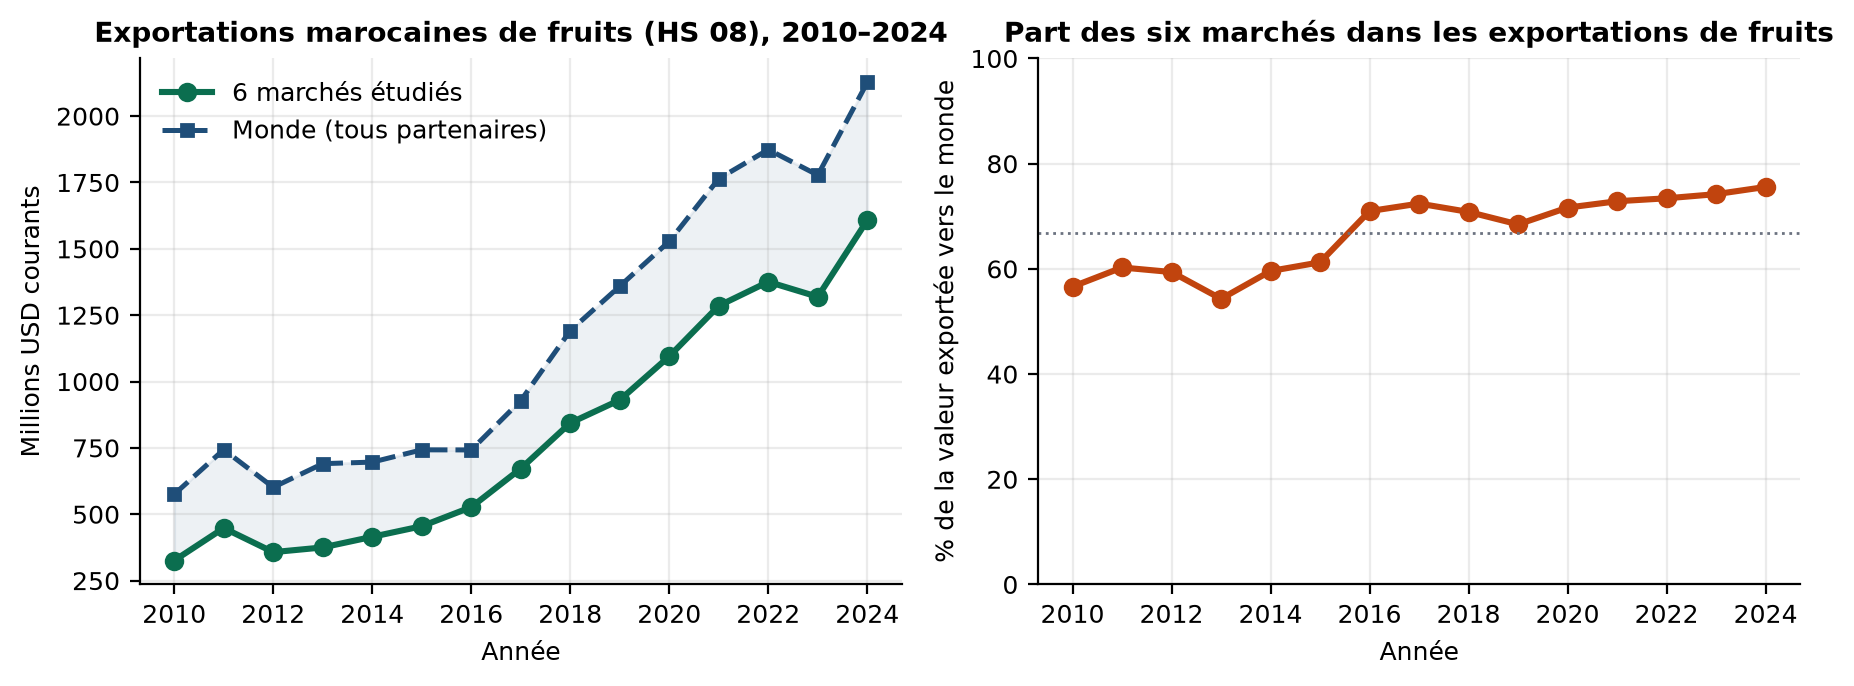
\includegraphics[width=\linewidth]{figures/fig01_dynamique_agregee.png}
\caption{Exportations marocaines de fruits vers les six marchés et vers le monde, et part des six marchés.}\label{fig:fig1}
\end{figure}

La valeur exportée vers les six marchés passe de 326\MUSD{} en 2010 à
1\,608\MUSD{} en 2024, soit une multiplication par 4,9 et un taux de croissance
annuel moyen de 12,1\,\%. La progression est continue, avec une accélération
nette après 2017 et un plateau en 2023 (recul de la demande européenne et effet
de base après la flambée de 2022). Les six marchés captent 56,6\,\% des
exportations marocaines de fruits en 2010 et 75,6\,\% en 2024 (66,8\,\% en
moyenne) : la zone étudiée est représentative, mais la dépendance à l'Europe
constitue un risque de concentration.

\begin{figure}[H]
\centering
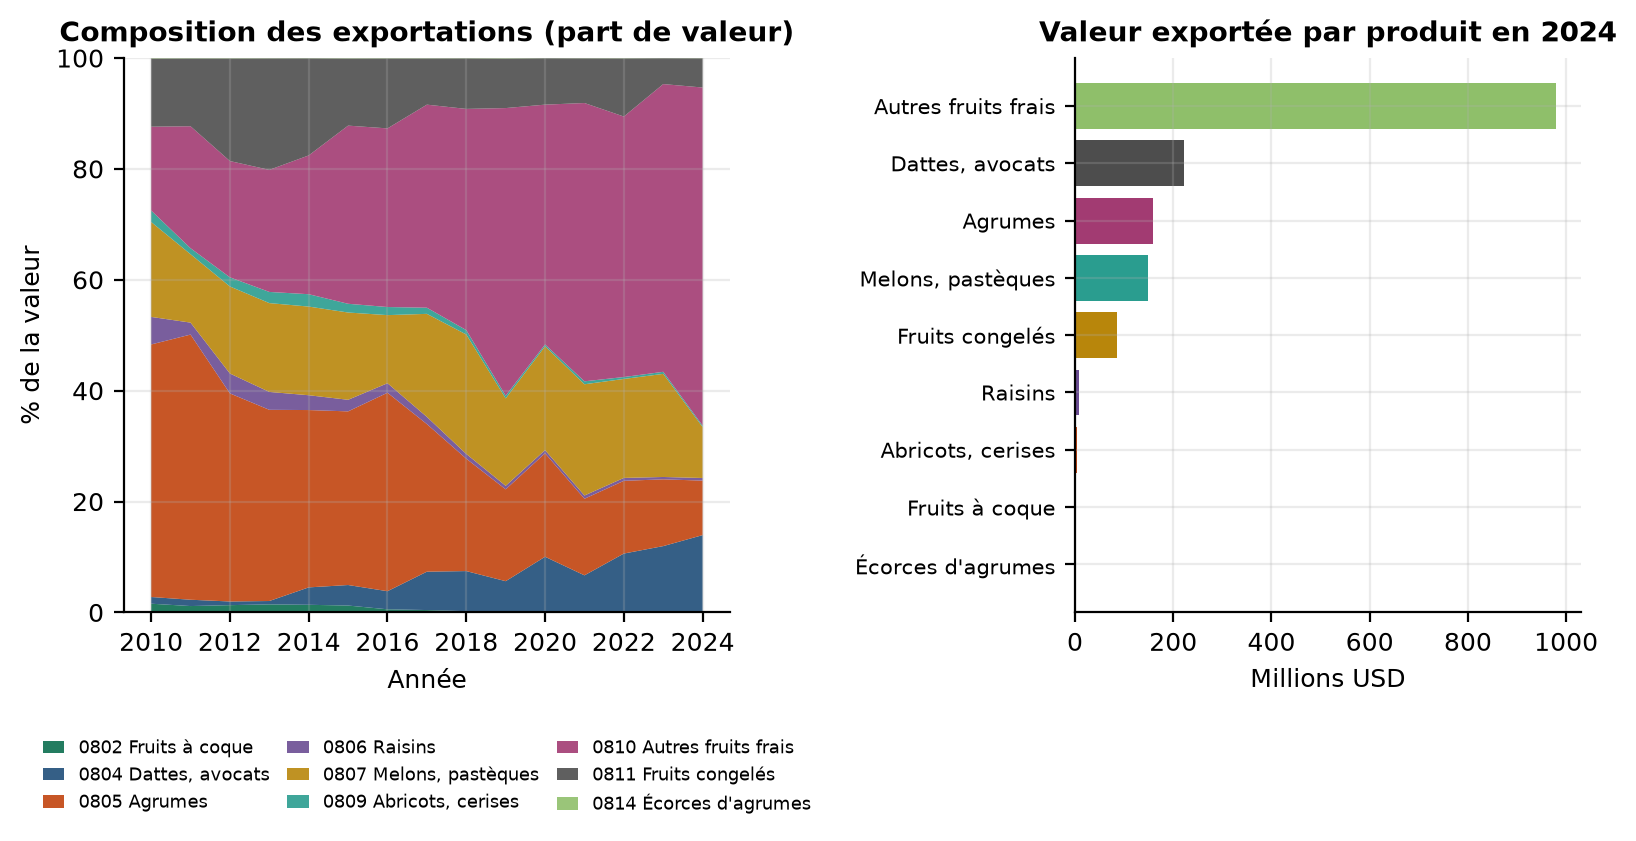
\includegraphics[width=\linewidth]{figures/fig02_structure_produits.png}
\caption{Composition des exportations de fruits par produit et valeur exportée en 2024.}\label{fig:fig2}
\end{figure}

La structure est dominée par les « autres fruits frais » (HS 0810 : fraises,
kiwis, grenades), qui représentent 61,0\,\% de la valeur en 2024, devant les
dattes et avocats (0804, 13,9\,\%), les agrumes (0805, 9,8\,\%) et les melons
et pastèques (0807, 9,2\,\%). Les agrumes, produit emblématique de la fiche
projet, ne pèsent donc qu'un dixième de la valeur du chapitre : la question
« prévoir les exportations d'agrumes » doit être traitée comme un cas
particulier d'un système plus large, ce qui justifie de modéliser le panel
produit $\times$ marché plutôt qu'une série isolée.

\begin{figure}[H]
\centering
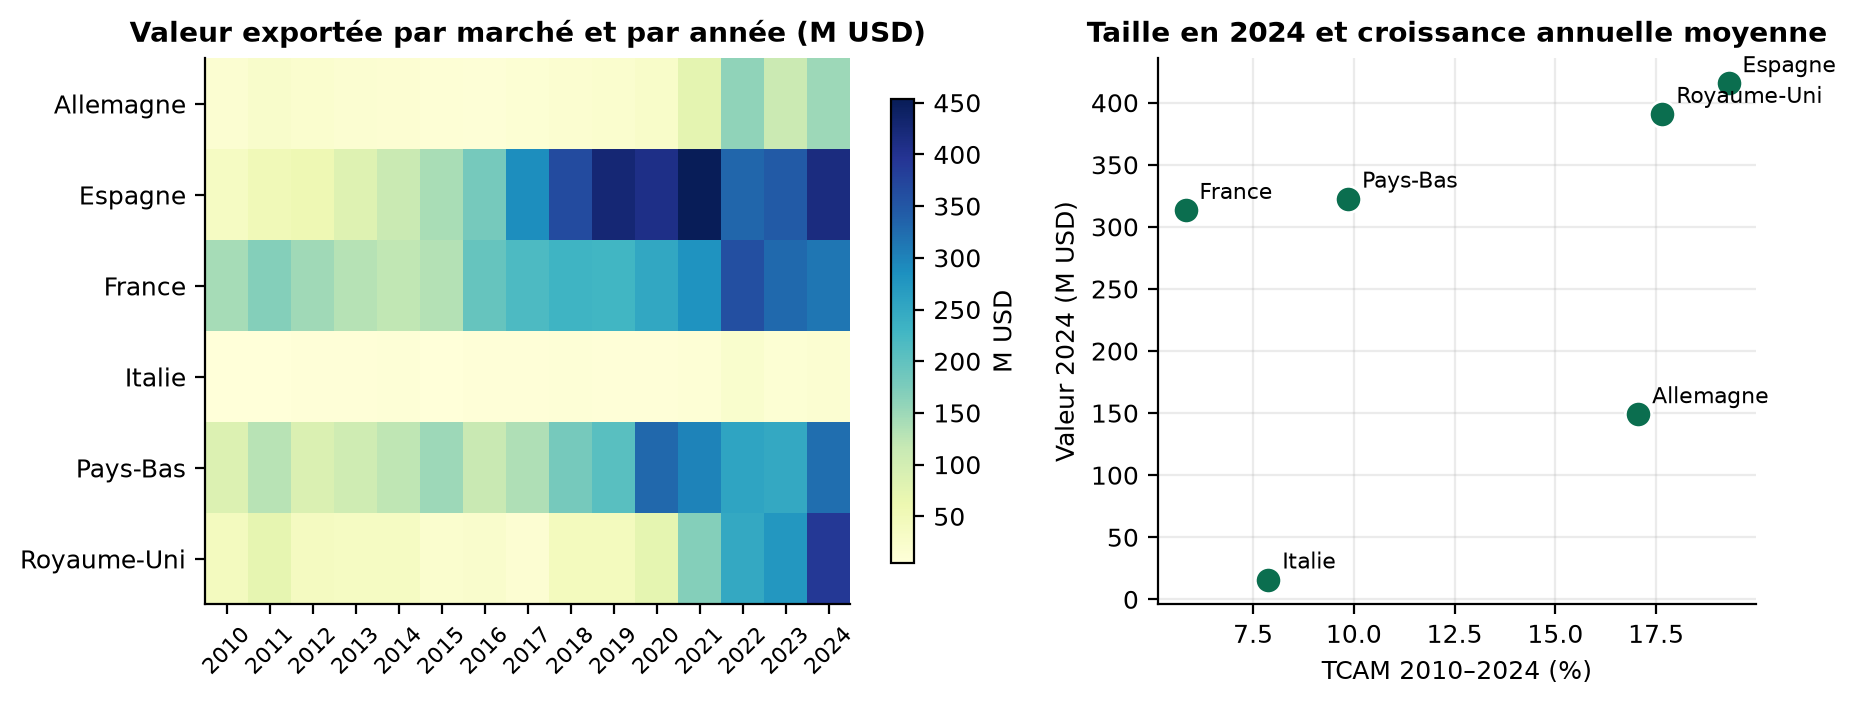
\includegraphics[width=\linewidth]{figures/fig03_marches.png}
\caption{Valeur exportée par marché et par année, et croisement taille 2024 / croissance moyenne.}\label{fig:fig3}
\end{figure}

Quatre marchés concentrent l'essentiel de la valeur en 2024 : l'Espagne
(415,6\MUSD), le Royaume-Uni (390,9), les Pays-Bas (322,6) et la France (313,5),
devant l'Allemagne (149,0) et l'Italie (15,9). Les trajectoires divergent
fortement : sur 2010--2024, l'Espagne (+19,3\,\% par an) et le Royaume-Uni
(+17,7\,\%) portent la croissance, tandis que la France, premier marché en 2010
(142,0\MUSD), ne progresse que de 5,8\,\% par an et perd des parts. Les
Pays-Bas jouent un rôle de hub de réexportation (Rotterdam), ce qui gonfle leur
poids dans les statistiques de destination.

\begin{figure}[H]
\centering
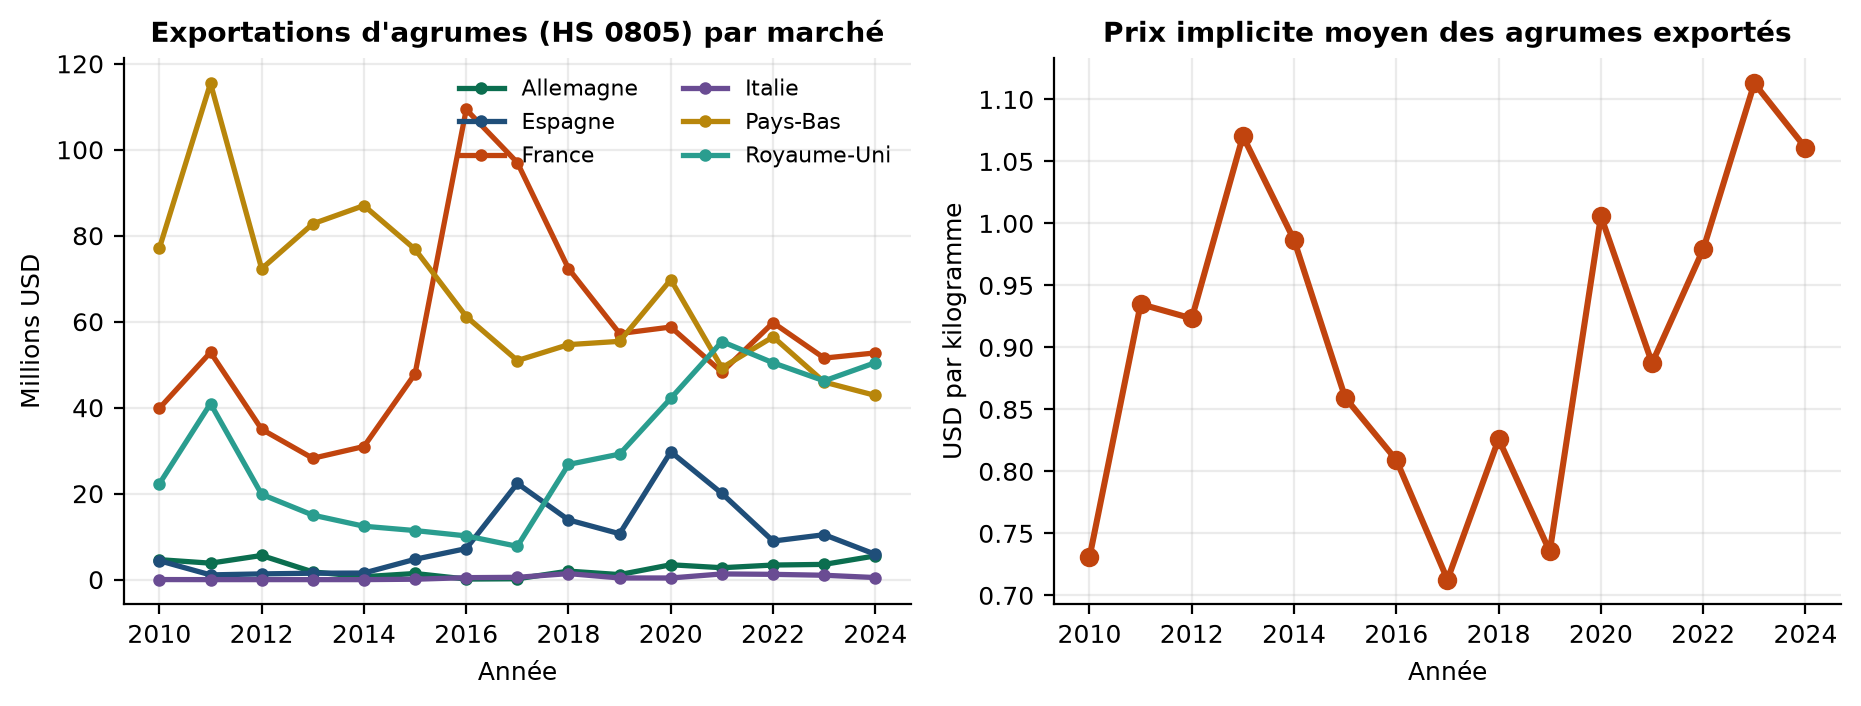
\includegraphics[width=\linewidth]{figures/fig04_agrumes.png}
\caption{Exportations d'agrumes (HS 0805) par marché et prix implicite moyen.}\label{fig:fig4}
\end{figure}

Le marché des agrumes est beaucoup plus volatil que le total : l'Espagne,
marginale jusqu'en 2015 (moins de 5\MUSD), bondit à 29,7\MUSD{} en 2020 puis
retombe à 5,9\MUSD{} en 2024 ; la France recule de 109,4\MUSD{} en 2016 à
52,7\MUSD{} en 2024 ; le Royaume-Uni double après 2020 (50,5\MUSD{} en 2024).
Le prix implicite des agrumes passe de 0,73 USD/kg en 2010 à 1,06 USD/kg en
2024 (+45\,\%), ce qui signale qu'une partie de la croissance en valeur est une
croissance de prix et non de volume.

\begin{figure}[H]
\centering
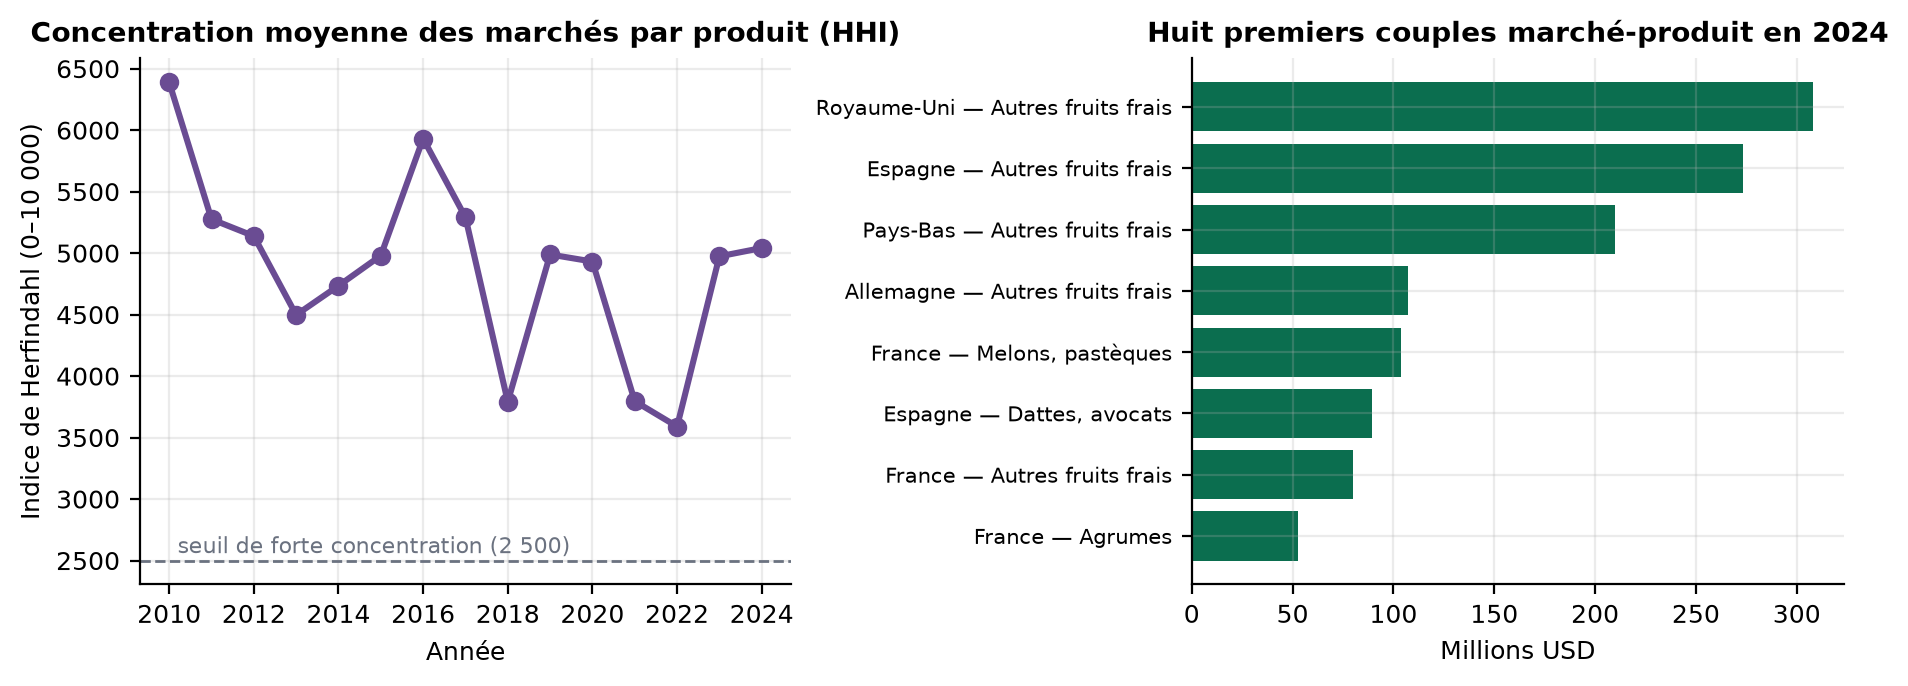
\includegraphics[width=\linewidth]{figures/fig05_concentration.png}
\caption{Concentration des marchés par produit (indice de Herfindahl) et principaux couples marché--produit en 2024.}\label{fig:fig5}
\end{figure}

L'indice de Herfindahl moyen reste très au-dessus du seuil de forte
concentration (5\,042 en 2024, contre 6\,388 en 2010) : pour chaque produit, un
ou deux marchés pèsent l'essentiel de la valeur. La concentration ne baisse pas
durablement, ce qui signifie que la diversification commerciale évoquée dans les
plans sectoriels ne se lit pas encore dans les données. Les trois premiers
couples (Royaume-Uni--0810, Espagne--0810, Pays-Bas--0810) concentrent à eux
seuls 49,2\,\% de la valeur exportée vers les six marchés en 2024.

\section{Méthodologie}\label{sec:method}

\subsection{Prétraitement et protocole sans fuite}

La cible est $y_{t+1}$, la valeur exportée du couple (marché, produit) l'année
suivante. Toutes les variables explicatives sont connues à la fin de l'année
$t$ : niveaux retardés, momentum, moyenne des trois derniers logarithmes, total
mondial du produit et part de marché. Aucune variable contemporaine de $t+1$,
aucun agrégat calculé avec l'année cible, aucune moyenne mobile centrée
n'est utilisée.

Le découpage est strictement temporel, en trois blocs :

\begin{itemize}[leftmargin=1.2cm]
\item \textbf{entraînement} : $t \leq 2019$ (cibles 2011--2020) ;
\item \textbf{validation glissante} : six fenêtres \emph{expanding window}
      (2016$\to$2017, \dots, 2021$\to$2022) pour choisir les hyperparamètres ;
\item \textbf{test final} : $t \in \{2022, 2023\}$, cibles 2023 et 2024,
      jamais utilisées avant la section~\ref{sec:resultats}.
\end{itemize}

Ce protocole reproduit la situation réelle : à chaque date, seul le passé est
disponible. Il évite la fuite temporelle, risque majeur signalé dans la fiche
projet.

\subsection{Modèles}

Quatre méthodes sont comparées.

\begin{description}[leftmargin=1.2cm,style=nextline]
\item[Persistance (référence).] $\hat y_{t+1} = y_t$. Benchmark naturel d'une
série de commerce ; la littérature sur les prévisions de commerce la considère
comme difficile à battre.
\item[Ridge.] Régression linéaire régularisée sur la variation
$\delta_t = \log(1+y_{t+1}) - \log(1+y_t)$, avec indicatrices marché et produit
et standardisation des variables numériques. Elle teste l'hypothèse d'une
dérive commune corrigée par des effets fixes.
\item[Forêt aléatoire.] 600 arbres, $min\_samples\_leaf \in \{3,8,15\}$,
$max\_features \in \{0,5\,;1\}$. Elle capture des seuils et des interactions
(par exemple un marché qui décroche après un pic).
\item[Gradient boosting.] \texttt{HistGradientBoostingRegressor} avec perte
absolue, $learning\_rate \in \{0,02\,;0,05\,;0,1\}$, 200 ou 500 itérations.
La perte absolue est alignée sur la métrique MAE.
\end{description}

Le prétraitement (indicatrices, standardisation) est encapsulé dans un
\texttt{Pipeline} scikit-learn, réajusté à chaque fenêtre : aucune statistique
calculée sur le test ne contamine l'entraînement.

\subsection{Métriques et équations}

Pour $n$ observations de test, avec $y_i$ la valeur réelle et $\hat y_i$ la
prévision :
\begin{equation}\label{eq:mae}
\mathrm{MAE}=\frac{1}{n}\sum_{i=1}^{n}\left|y_i-\hat y_i\right|,
\qquad
\mathrm{RMSE}=\sqrt{\frac{1}{n}\sum_{i=1}^{n}\left(y_i-\hat y_i\right)^2}.
\end{equation}
Dans l'équation~\eqref{eq:mae}, $y_i$ est la valeur exportée observée (USD),
$\hat y_i$ la valeur prévue, $n$ le nombre d'observations évaluées et
$|\cdot|$ la valeur absolue. Le RMSE pénalise davantage les grandes erreurs.

\begin{equation}\label{eq:wape}
\mathrm{WAPE}=\frac{\sum_{i=1}^{n}\left|y_i-\hat y_i\right|}
{\sum_{i=1}^{n}\left|y_i\right|}.
\end{equation}
Le WAPE de l'équation~\eqref{eq:wape} s'interprète comme une erreur relative
pondérée par la valeur : il donne du poids aux gros flux, ce qui correspond à
l'enjeu commercial. Un \emph{MASE} est ajouté, défini comme le rapport entre le
WAPE du modèle et celui de la persistance sur le même jeu ; une valeur
inférieure à 1 signale un gain par rapport à la référence.

\section{Résultats expérimentaux}\label{sec:resultats}

\subsection{Validation glissante et choix des hyperparamètres}

Le tableau~\ref{tab:grille} présente les meilleurs réglages par famille. La
persistance n'a pas d'hyperparamètre ; son WAPE moyen sur les six fenêtres est
de 0,297, avec une forte dispersion (de 0,193 pour 2021$\to$2022 à 0,366 pour
2020$\to$2021).

\begin{table}[H]
\centering
\caption{Meilleurs hyperparamètres par famille et WAPE moyen en validation glissante}\label{tab:grille}
\begin{tabular}{llr}
\toprule
Modèle & Hyperparamètres retenus & WAPE validation \\
\midrule
Persistance & --- & \textbf{0,297} \\
Forêt aléatoire & 600 arbres, feuille = 15, \texttt{max\_features} = 0,5 & 0,314 \\
Gradient boosting & $\eta=0,02$, 200 itérations, perte absolue & 0,314 \\
Ridge & $\alpha = 100$ & 0,381 \\
\bottomrule
\end{tabular}
\end{table}

Le Ridge est nettement distancé : la relation entre croissance passée et
croissance future n'est pas stable sur 2016--2022, et la régularisation forte
nécessaire pour stabiliser l'estimation le rapproche d'un modèle constant. Les
deux méthodes à base d'arbres font jeu égal, autour de 0,314.

\subsection{Évaluation hors échantillon}

Les modèles sont réajustés sur toutes les années $t \leq 2021$, puis évalués une
seule fois sur les cibles 2023 et 2024 (108 observations).

\begin{table}[H]
\centering
\caption{Comparaison des performances sur le test 2023--2024 (MAE et RMSE en M USD)}\label{tab:performances}
\small
\begin{tabular}{lrrrrr}
\toprule
Méthode & MAE & RMSE & WAPE test & WAPE valid. & MASE \\
\midrule
Persistance & 7,11 & 17,19 & 0,262 & \textbf{0,297} & 1,000 \\
Ridge & 10,71 & 29,53 & 0,395 & 0,381 & 1,506 \\
Forêt aléatoire & \textbf{6,90} & \textbf{16,37} & \textbf{0,255} & 0,314 & \textbf{0,971} \\
Gradient boosting & 8,00 & 18,06 & 0,295 & 0,314 & 1,125 \\
\bottomrule
\end{tabular}
\end{table}

\begin{figure}[H]
\centering
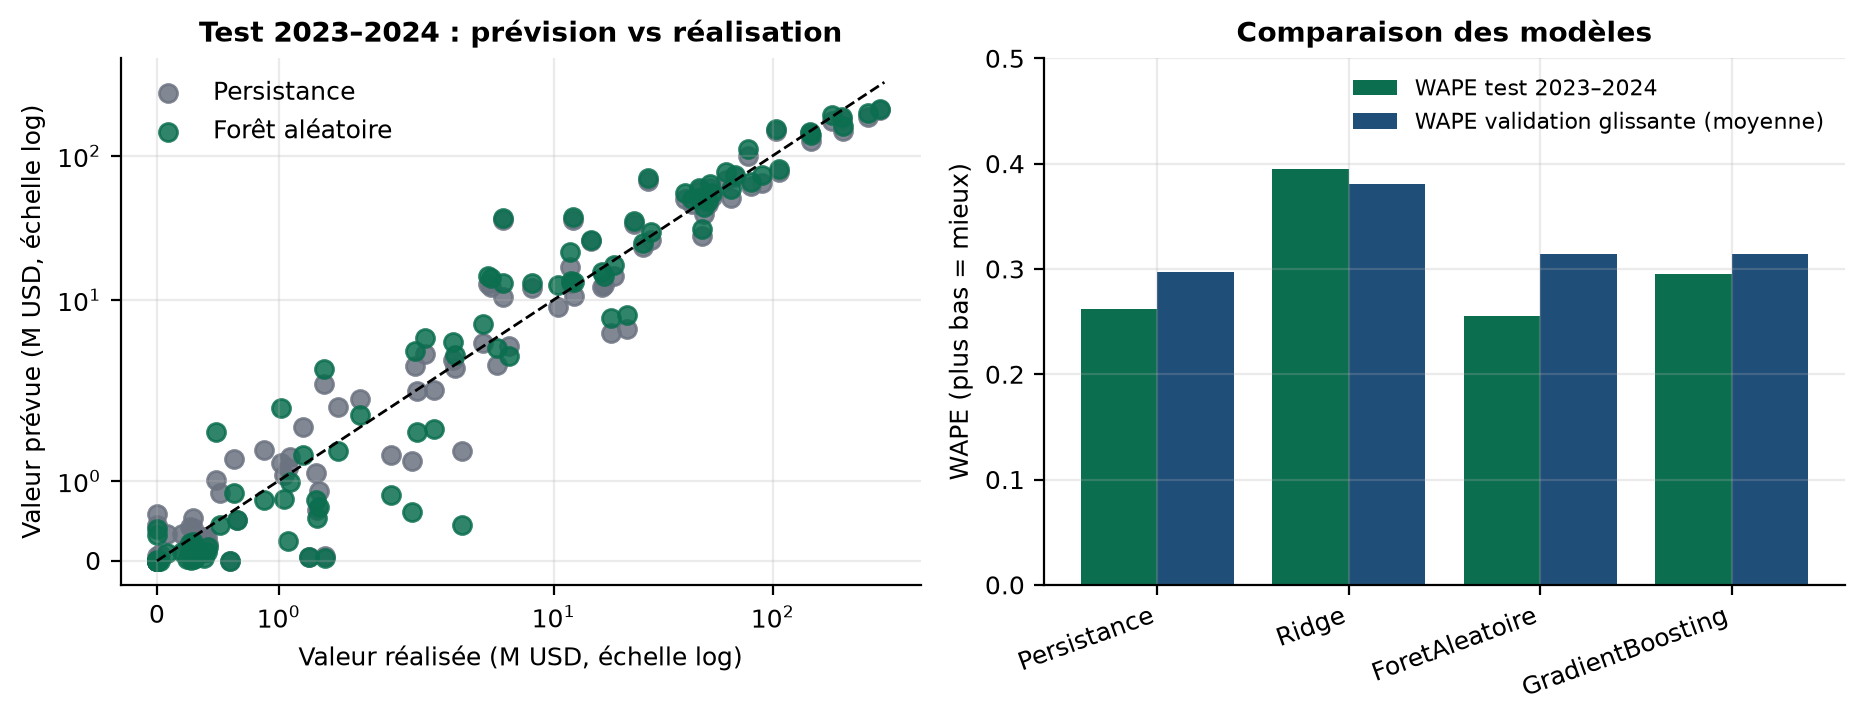
\includegraphics[width=\linewidth]{figures/fig06_comparaison_modeles.png}
\caption{Prévisions contre réalisations sur le test et comparaison des WAPE (validation et test).}\label{fig:fig6}
\end{figure}

Le tableau~\ref{tab:performances} et la figure~\ref{fig:fig6} livrent un
résultat nuancé. Sur le test, la forêt aléatoire devance la persistance
(WAPE 0,255 contre 0,262 ; MAE 6,90 contre 7,11\MUSD), soit un gain de 2,9\,\%
en erreur relative. Mais sur la validation glissante --- plus fiable car
calculée sur six fenêtres --- la persistance reste devant (0,297 contre 0,314).
Le gain du test n'est donc pas robuste : il dépend de la fenêtre et ne doit pas
être présenté comme une supériorité du modèle.

Le nuage de points montre par ailleurs que l'essentiel de l'erreur provient des
petits couples : les gros flux (au-dessus de 50\MUSD) sont bien alignés sur la
diagonale, alors que les flux inférieurs à 1\MUSD{} sont très dispersés. C'est
une propriété attendue : en échelle logarithmique, une erreur de quelques
centaines de milliers de dollars pèse autant qu'une erreur de plusieurs millions
sur un gros flux.

\subsection{Analyse des erreurs}

\begin{table}[H]
\centering
\caption{WAPE par marché sur le test 2023--2024}\label{tab:erreurs}
\begin{tabular}{lrrr}
\toprule
Marché & WAPE persistance & WAPE forêt aléatoire & Écart \\
\midrule
France & 0,182 & 0,199 & $+0,017$ \\
Royaume-Uni & 0,244 & \textbf{0,230} & $-0,014$ \\
Espagne & 0,267 & \textbf{0,233} & $-0,034$ \\
Pays-Bas & 0,273 & \textbf{0,238} & $-0,035$ \\
Allemagne & 0,426 & 0,478 & $+0,052$ \\
Italie & 0,650 & 0,935 & $+0,285$ \\
\bottomrule
\end{tabular}
\end{table}

L'analyse par marché est plus instructive que le résultat agrégé. La forêt
aléatoire améliore la prévision sur les trois marchés où les flux sont
importants et volatils (Espagne, Pays-Bas, Royaume-Uni) et la dégrade sur la
France, marché stable et bien prévu par la persistance, ainsi que sur les petits
marchés (Allemagne, Italie) où le bruit domine. Au niveau produit, le modèle
améliore le produit dominant 0810 (WAPE 0,214 contre 0,235) et les dattes et
avocats 0804 (0,243 contre 0,287), mais dégrade les agrumes 0805 (0,177 contre
0,128) : la série des agrumes est précisément celle où la persistance est la
plus difficile à battre.

\subsection{Importance des variables}

\begin{figure}[H]
\centering
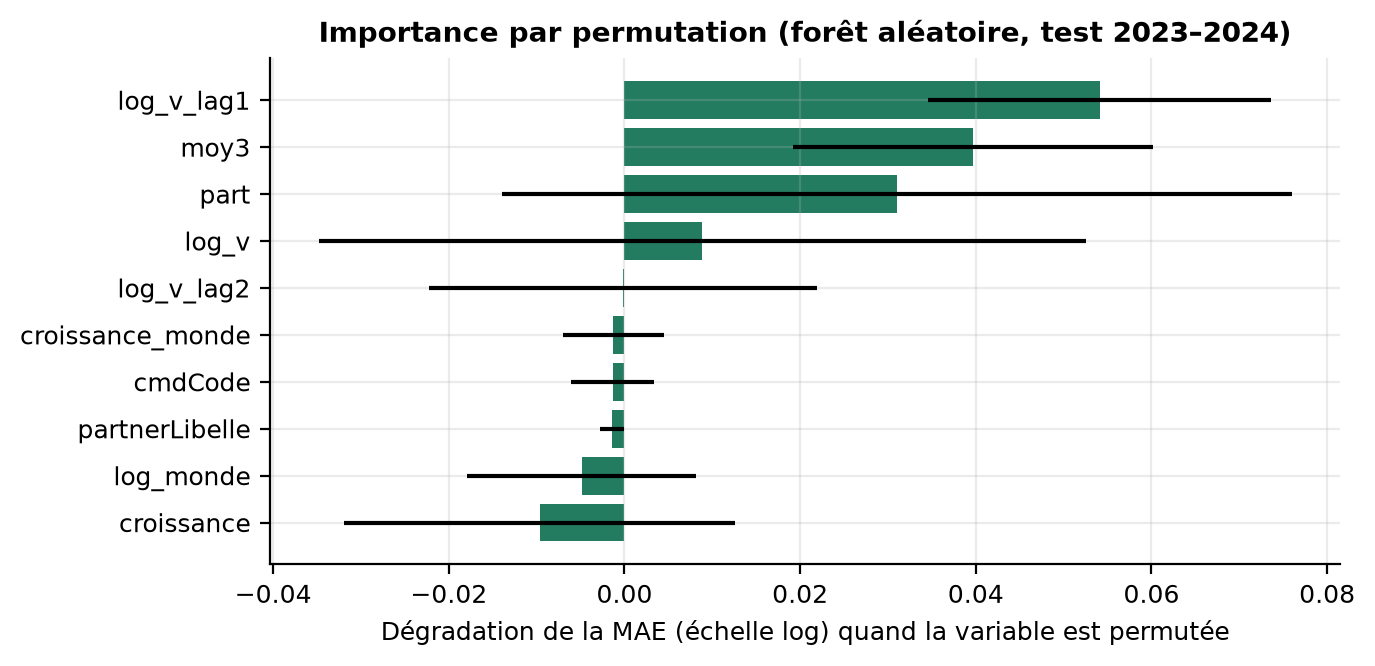
\includegraphics[width=0.78\linewidth]{figures/fig07_importance.png}
\caption{Importance par permutation des variables de la forêt aléatoire sur le test.}\label{fig:fig7}
\end{figure}

La figure~\ref{fig:fig7} confirme la lecture : la valeur retardée
(\texttt{log\_v\_lag1}, dégradation de MAE de 0,054) et la moyenne des trois
derniers logarithmes (\texttt{moy3}, 0,040) portent l'essentiel de
l'information. La part de marché apporte un complément (0,031), tandis que le
contexte mondial du produit (\texttt{log\_monde}, \texttt{croissance\_monde})
n'apporte presque rien. Autrement dit, \emph{le passé du couple
marché--produit contient déjà l'essentiel de ce que le modèle peut apprendre} :
c'est la définition même d'un processus proche d'une marche aléatoire.

\subsection{Sensibilité et robustesse}\label{sec:sensibilite}

\begin{table}[H]
\centering
\caption{Tests de sensibilité (WAPE sur le jeu évalué)}\label{tab:sensibilite}
\small
\begin{tabular}{>{\raggedright\arraybackslash}p{6.3cm}>{\raggedright\arraybackslash}p{3.2cm}rr}
\toprule
Scénario & Modèle & WAPE persistance & WAPE forêt \\
\midrule
Protocole principal & test 2023--2024 & 0,262 & 0,255 \\
S1 : zéros imputés exclus de l'entraînement & test 2023--2024 & --- & 0,253 \\
S2 : test élargi 2020--2024 & test 2020--2024 & 0,297 & 0,308 \\
S3 : hors produit dominant 0810 & test 2023--2024 & 0,298 & 0,288 \\
\bottomrule
\end{tabular}
\end{table}

Les conclusions résistent aux trois tests. Exclure les zéros imputés de
l'entraînement ne change pas le résultat (0,253 contre 0,255). Élargir le test
à 2020--2024 --- période marquée par la pandémie puis par l'inflation ---
inverse légèrement la hiérarchie au profit de la persistance. Retirer le produit
dominant 0810 ne modifie pas l'ordre de grandeur : le résultat n'est donc pas
porté par un seul couple.

\section{Discussion}\label{sec:discussion}

\subsection{Interprétation économique}

Le résultat central --- la persistance est un benchmark très difficile à battre
--- n'est pas un échec méthodologique, c'est une information économique. La
valeur exportée d'un couple (marché, produit) dépend de facteurs qui évoluent
lentement (structure de la demande, accords commerciaux, positions
concurrentielles) et de chocs qui, eux, ne sont pas prévisibles à partir du
passé (aléas climatiques, épisodes sanitaires, décisions de distribution). À
fréquence annuelle, le second terme domine le premier : la série se comporte
comme une marche aléatoire.

Trois enseignements opérationnels en découlent.

\begin{enumerate}[leftmargin=1.2cm]
\item \textbf{La valeur ajoutée du modèle n'est pas la prévision ponctuelle mais
la lecture des écarts.} Les couples où le modèle s'écarte fortement de la
persistance sont ceux qu'il faut examiner : changement de gamme, ouverture d'un
débouché, perte d'un client. C'est un outil de veille, pas un oracle.
\item \textbf{La croissance est largement une croissance de prix.} Le prix
implicite des agrumes augmente de 45\,\% entre 2010 et 2024, et le prix moyen
du chapitre 08 passe de 0,97 à 2,75 USD/kg. Un pilotage en valeur seule
surestime la performance commerciale ; il faut suivre les volumes.
\item \textbf{La concentration reste le premier risque.} L'indice de Herfindahl
ne baisse pas et les trois premiers couples pèsent la moitié de la valeur. La
diversification vers l'Allemagne, le Royaume-Uni ou les marchés hors UE est un
levier plus sûr qu'une optimisation de modèle.
\end{enumerate}

\subsection{Limites}

\begin{itemize}[leftmargin=1.2cm]
\item \textbf{Valeurs nominales.} Les montants sont en dollars courants ; aucune
déflation n'est appliquée, faute d'un indice de prix sectoriel homogène sur
2010--2024. Une partie de la croissance mesurée est de l'inflation.
\item \textbf{Séries courtes.} Quinze années annuelles, soit 648 observations
après construction des retards. Les modèles à base d'arbres sont bridés par
cette taille d'échantillon.
\item \textbf{Absence de saisonnalité.} La saisonnalité des agrumes et des
fruits rouges est invisible à fréquence annuelle ; c'est probablement la
première limite à lever.
\item \textbf{Hub néerlandais.} Les Pays-Bas réexportent une partie des flux :
la destination statistique n'est pas la destination finale.
\item \textbf{Zéros imputés.} Les cellules absentes sont traitées comme des flux
nuls ; le test S1 montre que cela ne change pas les conclusions, mais l'hypothèse
reste une simplification.
\item \textbf{Aucune causalité.} Les corrélations observées (prix, part de
marché) ne permettent pas d'inférer un effet causal. Une bonne précision
prédictive ne suffirait pas non plus à l'établir.
\end{itemize}

\section{Conclusion et perspectives}\label{sec:conclusion}

Le projet répond à sa question de recherche par un résultat négatif documenté :
sur des données annuelles, aucun des trois modèles testés ne bat la persistance
de manière robuste. La forêt aléatoire la devance de 2,9\,\% sur le test final
mais reste derrière en validation glissante ; le Ridge et le gradient boosting
sont distancés. Ce résultat est cohérent avec l'hypothèse H1 et avec la
littérature sur les prévisions de commerce.

L'hypothèse H2 est validée : la structure se déplace, avec la montée des fruits
hors agrumes (61,0\,\% de la valeur en 2024), le recul relatif de la France et
la montée de l'Espagne et du Royaume-Uni. L'hypothèse H3 est également validée :
le prix implicite des agrumes augmente de 45\,\% et le prix moyen du chapitre
presque triple, ce qui signifie qu'une part importante de la croissance en
valeur n'est pas une croissance en volume.

Trois prolongements sont prioritaires. D'abord, passer à une fréquence
mensuelle (Comtrade propose une fréquence \texttt{M}) pour capter la
saisonnalité et multiplier par douze le nombre d'observations. Ensuite, enrichir
le modèle avec des variables exogènes : prix de gros européens, indices de
production, taux de change MAD/EUR, indicateurs logistiques. Enfin, remplacer la
prévision ponctuelle par une prévision par intervalle et par scénario, plus
utile à un exportateur qu'un chiffre unique.

\paragraph{Projection 2025.} À titre indicatif, le modèle appliqué aux données
2024 projette 1\,771\MUSD{} d'exportations vers les six marchés en 2025
[1\,608 ; 1\,977] au seuil de 80\,\%, soit +10,2\,\% par rapport à 2024, avec
l'Espagne (471,5), le Royaume-Uni (414,0), les Pays-Bas (362,8) et la France
(345,2) en tête. Cette projection est un scénario de cadrage budgétaire, pas un
engagement : l'intervalle est construit à partir des erreurs relatives du
backtest roulant 2014--2024.

\begin{figure}[H]
\centering
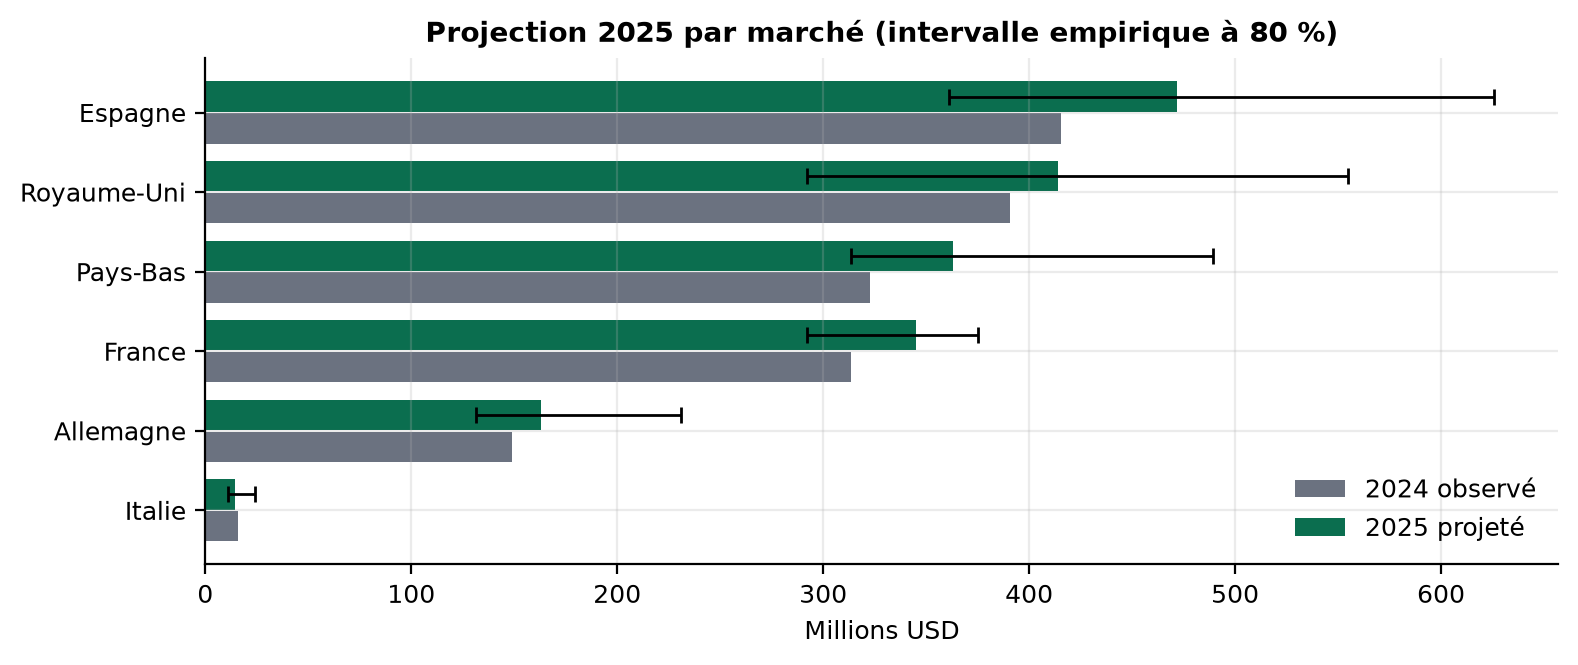
\includegraphics[width=0.85\linewidth]{figures/fig08_projection_2025.png}
\caption{Projection 2025 par marché et intervalle empirique à 80\,\%.}\label{fig:fig8}
\end{figure}

\begin{thebibliography}{9}
\bibitem{comtrade} Nations unies, Division statistique, \emph{UN Comtrade
Database --- API Documentation}. \url{https://uncomtrade.org/docs/un-comtrade-api/}.
Consulté le 31 octobre 2026.
\bibitem{comtradedata} Nations unies, \emph{UN Comtrade Database}.
\url{https://comtradeplus.un.org/}.
\bibitem{worldbank} Banque mondiale, \emph{Indicators API --- Documentation}.
\url{https://datahelpdesk.worldbank.org/knowledgebase/articles/889392}.
\bibitem{wto} Organisation mondiale du commerce, \emph{Tariff and Trade Data}.
\url{https://data.wto.org/en/dataset/wto_ttd}.
\bibitem{sklearn} F. Pedregosa \emph{et al.}, « Scikit-learn: Machine Learning in
Python », \emph{Journal of Machine Learning Research}, vol. 12, 2011,
p. 2825--2830.
\bibitem{hyndman} R. J. Hyndman et G. Athanasopoulos, \emph{Forecasting:
Principles and Practice}, 3\textsuperscript{e} éd., OTexts, 2021.
\bibitem{makridakis} S. Makridakis, E. Spiliotis et V. Assimakopoulos, « The M4
Competition: 100,000 time series and 61 forecasting methods », \emph{International
Journal of Forecasting}, vol. 36, n° 1, 2020, p. 54--74.
\end{thebibliography}

\appendix
\section{Reproductibilité}\label{ann:repro}

\begin{table}[H]
\centering
\caption{Éléments de reproductibilité}\label{tab:repro}
\begin{tabular}{ll}
\toprule
Élément & Valeur \\
\midrule
Graine aléatoire & 42 \\
Ordre d'exécution & \texttt{download\_comtrade.py} $\to$ \texttt{prepare\_data.py} $\to$ notebook \\
Requêtes API & 45 (15 années $\times$ 3 extractions), 0 échec \\
Données brutes & \texttt{data/raw/comtrade\_*.json} \\
Journal des requêtes & \texttt{data/processed/journal\_extractions.csv} \\
Résultats & \texttt{data/processed/resultats\_modeles.json} \\
Notebook & \texttt{notebooks/projet12\_exportations\_agroalimentaires.ipynb} \\
Figures & \texttt{figures/fig01} à \texttt{fig08}, 200 dpi \\
Versions & Python 3.14.8, numpy 2.x, pandas 3.1.0, scikit-learn 1.9.1 \\
\bottomrule
\end{tabular}
\end{table}

Le notebook s'exécute de bout en bout (\emph{Run all}) sans erreur. Les scripts
d'acquisition et de préparation sont séparés de l'analyse pour que celle-ci
reste lisible ; les deux étapes sont documentées dans le \texttt{README.md}.

\section{Journal des contributions et déclaration d'IA}

\begin{table}[H]
\centering
\caption{Journal des contributions du binôme}\label{tab:contrib}
\begin{tabular}{lcc}
\toprule
Tâche & Étudiant 1 & Étudiant 2 \\
\midrule
Cadrage, question de recherche & $\square$ & $\square$ \\
Extraction API et journal & $\square$ & $\square$ \\
Nettoyage et dictionnaire & $\square$ & $\square$ \\
Analyse exploratoire et figures & $\square$ & $\square$ \\
Modélisation et validation & $\square$ & $\square$ \\
Tests de sensibilité & $\square$ & $\square$ \\
Rédaction \LaTeX{} et soutenance & $\square$ & $\square$ \\
\bottomrule
\end{tabular}
\end{table}

\textbf{Déclaration d'usage d'outils d'IA.} Conformément aux règles de
l'établissement, l'usage d'un assistant de programmation pour la mise en forme
du code et la relecture rédactionnelle doit être déclaré et vérifié par les deux
membres du binôme. Les données, les résultats et les interprétations restent de
la responsabilité des auteurs. Aucune donnée n'a été simulée ni inventée.

\end{document}
